\section{Anchor-Decoupled Evaluation Protocol}
\label{sec:method}


\begin{figure*}[t]
\centering
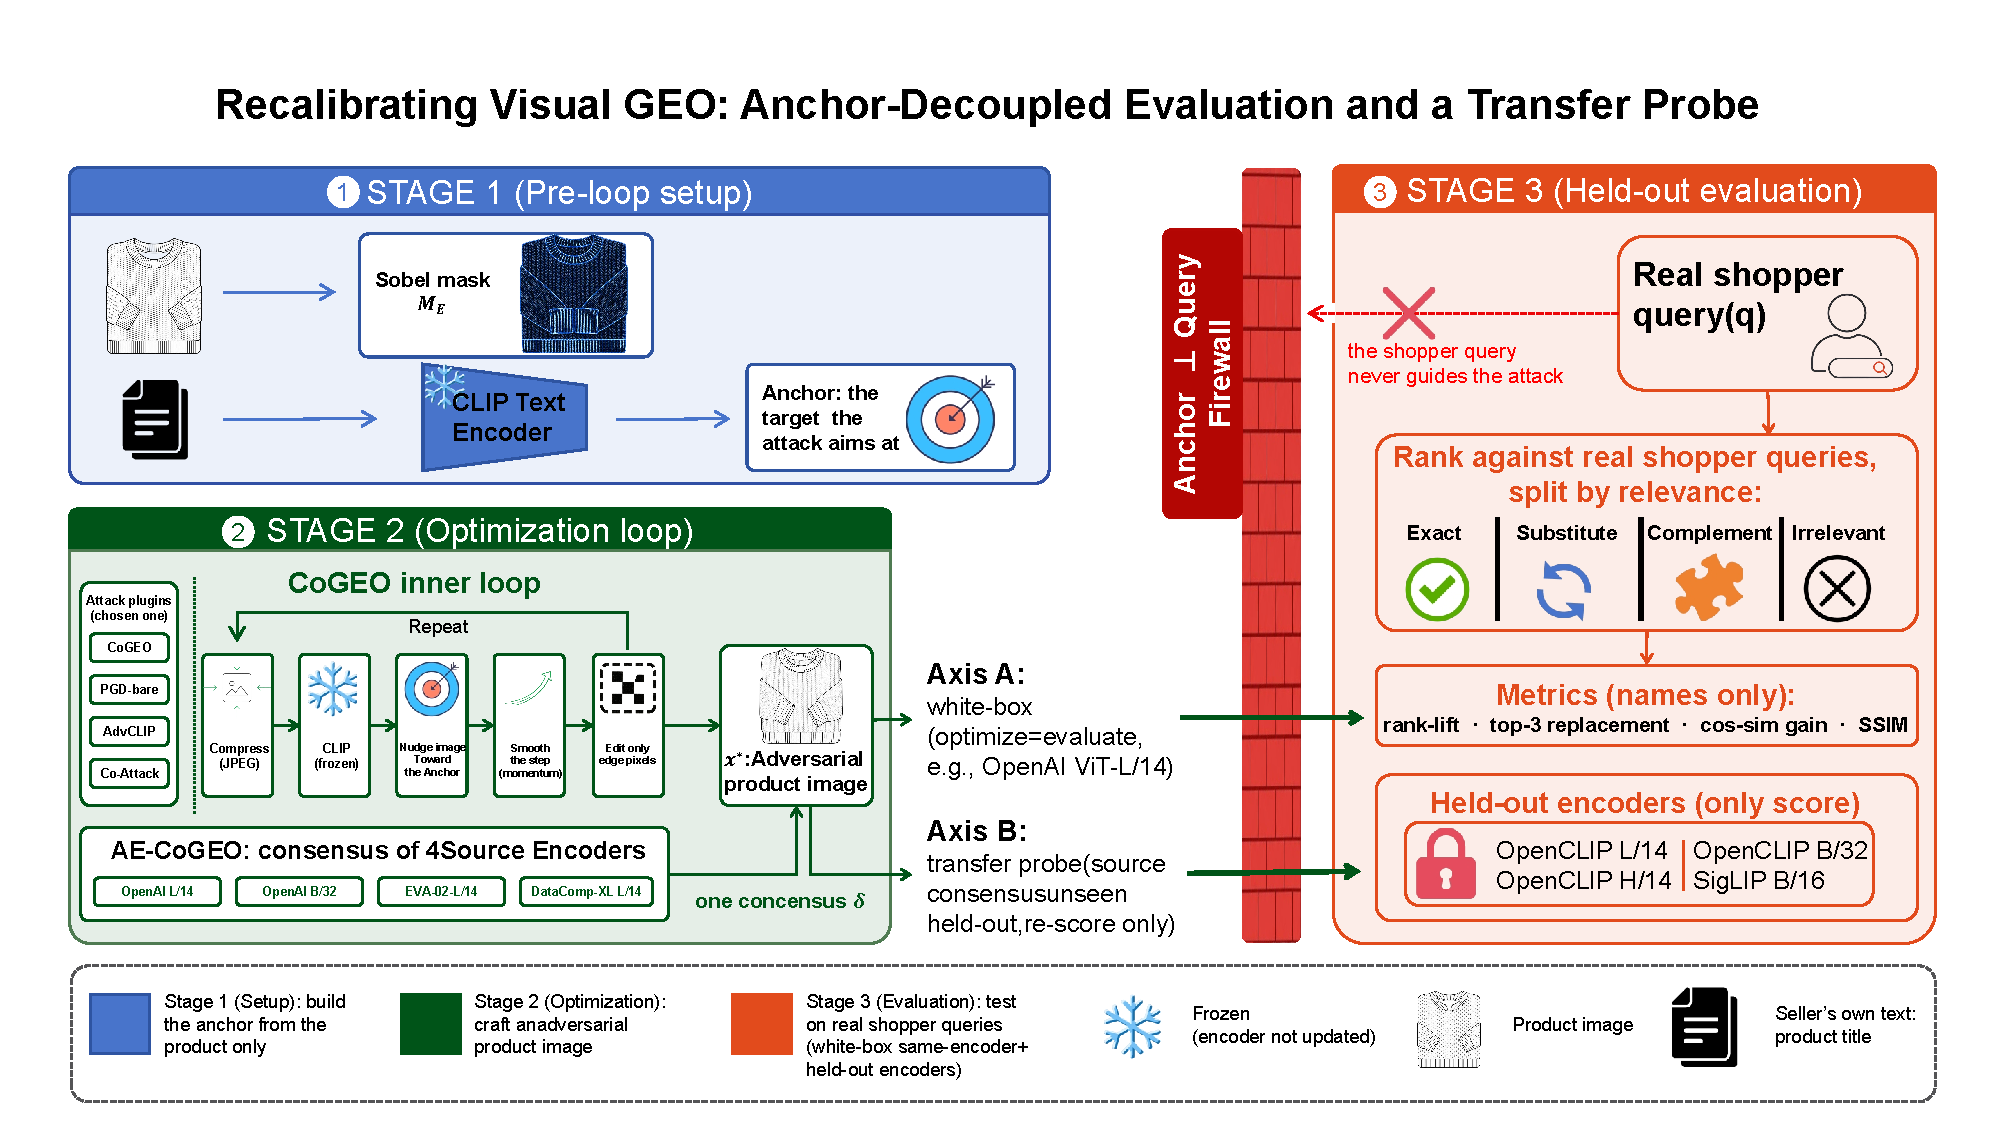
\includegraphics[width=0.85\textwidth]{figures/fig_framework.pdf}
\caption{Anchor-decoupled evaluation protocol with a cross-encoder transfer probe, instantiated for CoGEO. \textbf{Stage~1} precomputes the seller anchor $v_{\mathrm{anchor}}{=}E_T(t_p^{\star})$ from the product title and a Sobel-edge mask $M_E$ (top-$40\%$ gradient pixels); $v_{\mathrm{anchor}}$ depends on the product image alone, never on a shopper query. \textbf{Stage~2} runs the CoGEO inner loop---JPEG-compress, encode with the frozen CLIP tower, nudge toward the anchor, smooth with momentum, edit only masked edge pixels---for $K{=}200$ iterations at $\varepsilon{=}16/255$; baselines PGD-bare, AdvCLIP and Co-Attack drop or replace individual boxes. Two orthogonal axes, not competing attacks: \emph{Axis~A} optimizes against a single white-box encoder; \emph{Axis~B} (AE-CoGEO) against a four-source consensus loss $L_{\mathrm{ens}}{=}-\tfrac{1}{|\mathcal{S}|}\sum_{j}\cos(E_I^{(j)}(\tilde{x}),E_T^{(j)}(t_p^{\star}))$. \textbf{Stage~3} scores the frozen image against unseen ESCI shopper queries across the four cohorts (E/S/C/I) and re-scores Axis~B---no re-attack---on four held-out encoders. The shopper query never crosses the Anchor-Decoupled Query Firewall. Snowflakes mark frozen modules.}
\Description{Three-stage anchor-decoupled pipeline with a transfer probe. Stage one builds a frozen text anchor from the product title together with a Sobel gradient mask; the anchor depends only on the product image, never on the shopper query. Stage two runs a five-step perturbation loop (differentiable JPEG, frozen image encoding, anchor-alignment cosine loss, momentum gradient, masked projection) and splits into two orthogonal axes: a white-box axis against a single encoder, and a transfer axis (AE-CoGEO) that optimizes a four-encoder consensus loss over optimize-only source encoders. Stage three scores the frozen image against unseen shopper queries across four relevance cohorts and re-scores the transfer axis on four held-out encoders without re-attacking; the query is separated from the optimization path by an anchor-decoupled query firewall.}
\label{fig:framework}
\end{figure*}

\subsection{\texorpdfstring{The anchor$\perp$query invariant}{The anchor-perpendicular-query invariant}}
\label{sec:method:invariant}

Let $x_p$ denote a product image, $q$ a shopper query in natural language, $E_I$ and $E_T$ the image and text encoders of a CLIP-style retriever~\cite{radford2021clip,jia2021scaling,cherti2023reproducible}, and $v_{\text{anchor}}(x_p) \in \mathbb{R}^d$ a target text embedding used to drive a perturbation $\delta$ such that $E_I(x_p + \delta)$ moves toward $v_{\text{anchor}}(x_p)$.

We require that, for every $(q, x_p)$ pair used in evaluation,
\begin{equation}
v_{\text{anchor}}(x_p)\ \text{is a function of}\ x_p\ \text{alone,}\ \text{not of}\ q.
\label{eq:invariant}
\end{equation}
Concretely, $v_{\text{anchor}}$ may be the CLIP text encoding of the product category, of a VLM description of $x_p$ (varied across BLIP, BLIP-2, LLaVA-1.5, Qwen2-VL, and Qwen2.5-VL in the released artifact), or of the product title; in all cases it depends only on the seller-side description. The query $q$ enters only at evaluation time, when we measure rank-lift, top-3 replacement, and held-out cosine similarity gains under $q$.

This invariant is the operational definition of an honest visual-GEO evaluation: when the eval query is itself derived from $v_{\text{anchor}}$, the similarity gain is structurally inflated relative to held-out retrieval impact. We enforce \eqref{eq:invariant} at the code level across all four families with a compact reference verifier ($\sim$60 lines, released artifact) that statically rejects any query-like attack parameter and dynamically checks that the perturbation is byte-identical across swapped eval queries under a fixed seed.

\subsection{Pre-flight monotonicity gate}
\label{sec:method:noop}

Before any adversarial perturbation, the chosen retriever must demonstrate that human-graded relevance labels are discriminable in its embedding space. Writing $\overline{\cos}_{\ell} = \mathrm{mean}_{(q,x_p)\in\ell}\bigl[\cos(E_I(x_p),\,E_T(q))\bigr]$ for the mean no-perturbation cosine over a cohort $\ell$, we require that on a balanced sample of $(q, x_p, \ell)$ triples spanning the four ESCI relevance classes Exact (E), Substitute (S), Complement (C), Irrelevant (I), the gate
\begin{equation}
\overline{\cos}_{\ell=E} - \overline{\cos}_{\ell=I} \;\geq\; 0.05
\label{eq:noop_gate}
\end{equation}
holds.
A retriever that fails \eqref{eq:noop_gate} cannot serve as an evaluation substrate: no adversarial pressure is measurable against an embedding that cannot already separate Exact-match from Irrelevant pairs. We read $0.05$ as a qualitative admissibility floor, not a calibrated statistic: a conservative margin that the canonical CoGEO retriever (ViT-L/14, gap $0.0533$) clears and a markedly weaker substrate (ViT-B/32, $0.0405$) does not, with both satisfying $E\!>\!S\!>\!C\!>\!I$ monotonicity. The evaluation substrate (ViT-L/14) is fixed independently as the canonical retriever, so no downstream result depends on the exact floor value. On failure, the protocol mandates a backbone swap before optimization.

\subsection{Four-way attack pass}
\label{sec:method:attacks}

Within the invariant, four white-box attack families are evaluated at a matched perturbation budget $\eps = 16/255$, the cross-family normalization point at which all four families separate cleanly (not a claim that it is the only deployment-relevant budget; the budget-dependence is examined in \S\ref{sec:analysis:eps}):

\paragraph{CoGEO} Per-image projected gradient descent~\cite{madry2018pgd,goodfellow2015fgsm} on $x_p$ with momentum (MI-FGSM~\cite{dong2018mifgsm}), Sobel-edge mask restricting perturbation to high-gradient regions, environment simulation through a differentiable JPEG layer~\cite{shin2017diffjpeg} together with input-diversity~\cite{xie2019dim} and scale-invariant~\cite{lin2020sim} transformations, and product-title $v_{\text{anchor}}$; CoGEO is the attack we propose and the primary subject of the held-out evaluation. Adapting it to the anchor-decoupled protocol fixes three design choices, each settled by an ablation in the released artifact: a hard top-$40\%$ Sobel-gradient mask (vs.\ a soft min-max-normalized mask floored at $0.1$), differentiable JPEG at $Q{=}75$ (vs.\ $Q{=}85$), and translation-invariant smoothing omitted, as it gave no significant lift under the anchor$\perp$query setting.

Formally, let $x_p^{(k)}$ denote the listing image at iteration $k$ (with $x_p^{(0)}{=}x_p$). The Sobel edge mask
\begin{equation}
M_E \;=\; \mathbf{1}\!\bigl[\,|\nabla_{\mathrm{Sobel}}\,x_p|\;\geq\;q_{0.6}(|\nabla_{\mathrm{Sobel}}\,x_p|)\,\bigr]
\label{eq:sobel_mask}
\end{equation}
selects the top-$40\%$ gradient pixels (threshold $q_{0.6}$, the $60$-th percentile of edge magnitude) and is computed once per image. At each iteration $k$, CoGEO applies a differentiable JPEG layer at quality $Q{=}75$ to make the attack compression-aware, embeds the result with the frozen CLIP image encoder, and forms the anchor-alignment loss
\begin{equation}
L^{(k)} \;=\; -\,\cos\!\bigl(\,E_I(\mathrm{diffJPEG}_{Q=75}(x_p^{(k)})),\; v_{\mathrm{anchor}}\,\bigr).
\label{eq:anchor_loss}
\end{equation}
The signed gradient is smoothed by a momentum buffer with $\mu=1.0$ following the original MI-FGSM formulation~\cite{dong2018mifgsm}:
\begin{equation}
g^{(k+1)} \;=\; \mu\,g^{(k)} \;+\; \frac{\nabla_{x}\,L^{(k)}}{\lVert\nabla_{x}\,L^{(k)}\rVert_1}, \quad \mu = 1.0,
\label{eq:mifgsm_momentum}
\end{equation}
The masked signed-momentum step (step size $\alpha = 4/255$) is then projected onto the $\ell_\infty$ $\varepsilon$-ball $\mathcal{B}_\infty(x_p,\varepsilon){=}\{x:\lVert x-x_p\rVert_\infty{\leq}\varepsilon\}$:
\begin{equation}
x_p^{(k+1)} \;=\; \Pi_{\mathcal{B}_\infty(x_p,\,\varepsilon)}\!\Bigl( x_p^{(k)} - \alpha \cdot \mathrm{sign}\bigl(M_E \odot g^{(k+1)}\bigr) \Bigr).
\label{eq:masked_step}
\end{equation}
After $K{=}200$ iterations, $x_p^{\star}$ is the adversarial image evaluated against the held-out query in \S\ref{sec:method:metrics}.

\paragraph{PGD-bare} The same product-title $v_{\text{anchor}}$ as CoGEO but without the Sobel mask, environment simulation, or momentum, recovering the classical signed-step PGD baseline of~\cite{madry2018pgd} and isolating the anchor's contribution from the engineering layered on top.

\paragraph{AdvCLIP} A query-agnostic universal adversarial patch~\cite{moosavidezfooli2017uap,thys2019adversarialpatches} trained on the CLIP image encoder~\cite{zhou2023advclip} over 30 epochs with budget $\eps = 16/255$, applied to each $x_p$ at evaluation. AdvCLIP requires no per-image gradient pass at deployment time.

\paragraph{Co-Attack} A cross-modal alternating attack~\cite{zhang2022coattack} that interleaves an $L_\infty$ image perturbation ($\eps = 16/255$) and an $L_2$ text-anchor perturbation ($\eps_v = 0.1$) over 200 iterations. The text branch operates on the seller-side anchor only, never on $q$, so the invariant is preserved.

All four pipelines take only $x_p$ as optimization input; the held-out ESCI query never enters any optimization gradient, verified at the code level.

The CoGEO inner loop is fully specified by Eqs.~\eqref{eq:sobel_mask}--\eqref{eq:masked_step}; the full evaluation-pass pseudocode is in the released artifact.

\subsection{AE-CoGEO: a cross-encoder-consensus transfer probe}
\label{sec:method:aecogeo}

The four-way comparison above is a \emph{white-box} measurement: the encoder that drives the perturbation also scores it. This bounds one axis --- how far an attacker can move the ranking of a retriever it fully controls --- but leaves unmeasured the realistic deployment axis, where the platform retriever is an \emph{unseen} encoder the attacker never optimized against. We introduce \textbf{AE-CoGEO} (Anchor-decoupled Ensemble CoGEO) to measure this second axis.

AE-CoGEO keeps both protocol commitments of CoGEO unchanged --- the perturbation is \emph{query-free} and \emph{anchor-decoupled}, so the held-out shopper query never enters optimization (\eqref{eq:invariant}) --- and adds a single mechanism: instead of aligning to one encoder, it optimizes one perturbation against the \emph{consensus} of a source set of encoders $\mathcal{S}=\{(E_I^{(j)}, E_T^{(j)})\}_{j=1}^{m}$ ($m=|\mathcal{S}|=4$ source encoders). Writing $t_p^{\star}=\textsc{SellerAnchor}(x_p)$ for the seller-side anchor text and $\tilde{x}=\mathrm{diffJPEG}_{Q}(x_p+\delta)$, the anchor-alignment loss is averaged over the source set,
\begin{equation}
L_{\mathrm{ens}}(\delta) = -\frac{1}{m}\sum_{j=1}^{m} \cos\bigl(E_I^{(j)}(\tilde{x}),\, E_T^{(j)}(t_p^{\star})\bigr),
\label{eq:ens_loss}
\end{equation}
and the masked MI-FGSM update of \eqref{eq:mifgsm_momentum}--\eqref{eq:masked_step} is applied to $\nabla_\delta L_{\mathrm{ens}}$ without change, so $\delta$ raises anchor alignment \emph{simultaneously} across architectures rather than overfitting one encoder's geometry. Ensemble optimization is a standard transferability route~\cite{papernot2017transferable,dong2018mifgsm,xie2019dim}; AE-CoGEO's increment is combining it diagnostically with the query-free, anchor-decoupled constraint visual GEO imposes.

Source and held-out encoders are strictly disjoint: the source set is $\mathcal{S}=\{$OpenAI ViT-L/14, OpenAI ViT-B/32, EVA-02-L/14, DataComp-XL ViT-L/14$\}$ and the held-out set is $\{$OpenCLIP-L/14, -H/14, -B/32 (all LAION-2B), SigLIP ViT-B/16$\}$, with no shared checkpoint and no shared pretraining corpus. Every other setting --- $\eps=16/255$, $K=200$, Sobel mask, differentiable-JPEG and input-diversity environment simulation, and product-title anchor --- is identical to the single-encoder CoGEO arm, so any change in held-out behavior is attributable to the consensus mechanism alone.

CoGEO and AE-CoGEO thus instrument two orthogonal axes of the same threat --- the white-box and transfer ceilings --- with AE-CoGEO the calibrated transfer probe; \S\ref{sec:analysis:transfer} reports the measurement.

\subsection{Per-cohort decomposition and significance}
\label{sec:method:metrics}

For each adversarial image $x_p^* = x_p + \delta$ we compute four metrics against the held-out query~$q$: \emph{rank-lift} $\mathrm{rank}(x_p, q) - \mathrm{rank}(x_p^*, q)$, the positions $x_p^*$ rises for $q$; \emph{top-3 replacement rate}, the fraction of pairs where $x_p^*$ enters the top $3$ while $x_p$ did not; \emph{held-out} $\Delta_{\mathrm{clip\_sim}} = \cos(E_I(x_p^*), E_T(q)) - \cos(E_I(x_p), E_T(q))$, the direct CLIP-similarity gain under $q$; and \emph{SSIM} between $x_p$ and $x_p^*$ at the retriever's native resolution, the stealth at the regime industrial retrieval consumes. Every metric is then \emph{decomposed} per cohort over the four ESCI relevance classes. Aggregate means across all pairs are reported alongside per-cohort means, never as a substitute. We further compute a paired Wilcoxon signed-rank test for each of the $\binom{4}{2}=6$ method pairs on the same $(q, x_p)$ index, so each pairwise comparison is verifiable independently of any cohort selection.

